\documentclass[border=12pt]{standalone}
\usepackage[T1]{fontenc}
\usepackage{helvet}
\renewcommand{\familydefault}{\sfdefault}
\usepackage{amsmath}
\usepackage{tikz}
\usetikzlibrary{positioning,arrows.meta,calc,fit,backgrounds,shapes.geometric,shapes.misc}

% palette
\definecolor{spinefill}{RGB}{232,234,238}
\definecolor{spinedraw}{RGB}{110,118,130}
\definecolor{liverfill}{RGB}{246,247,249}
\definecolor{liverdraw}{RGB}{168,175,184}
\definecolor{teald}{RGB}{13,110,122}
\definecolor{tealfill}{RGB}{223,239,240}
\definecolor{amber}{RGB}{193,118,18}
\definecolor{amberfill}{RGB}{250,240,222}
\definecolor{inkc}{RGB}{33,38,46}
\definecolor{salmon}{RGB}{193,110,95}
\definecolor{salmonfill}{RGB}{244,225,220}

% badges
\newcommand{\bnew}{\colorbox{teald}{\textcolor{white}{\scriptsize\bfseries NEW}}\hspace{2pt}}
\newcommand{\bchg}{\colorbox{amber}{\textcolor{white}{\scriptsize\bfseries CHANGED}}\hspace{2pt}}

\begin{document}
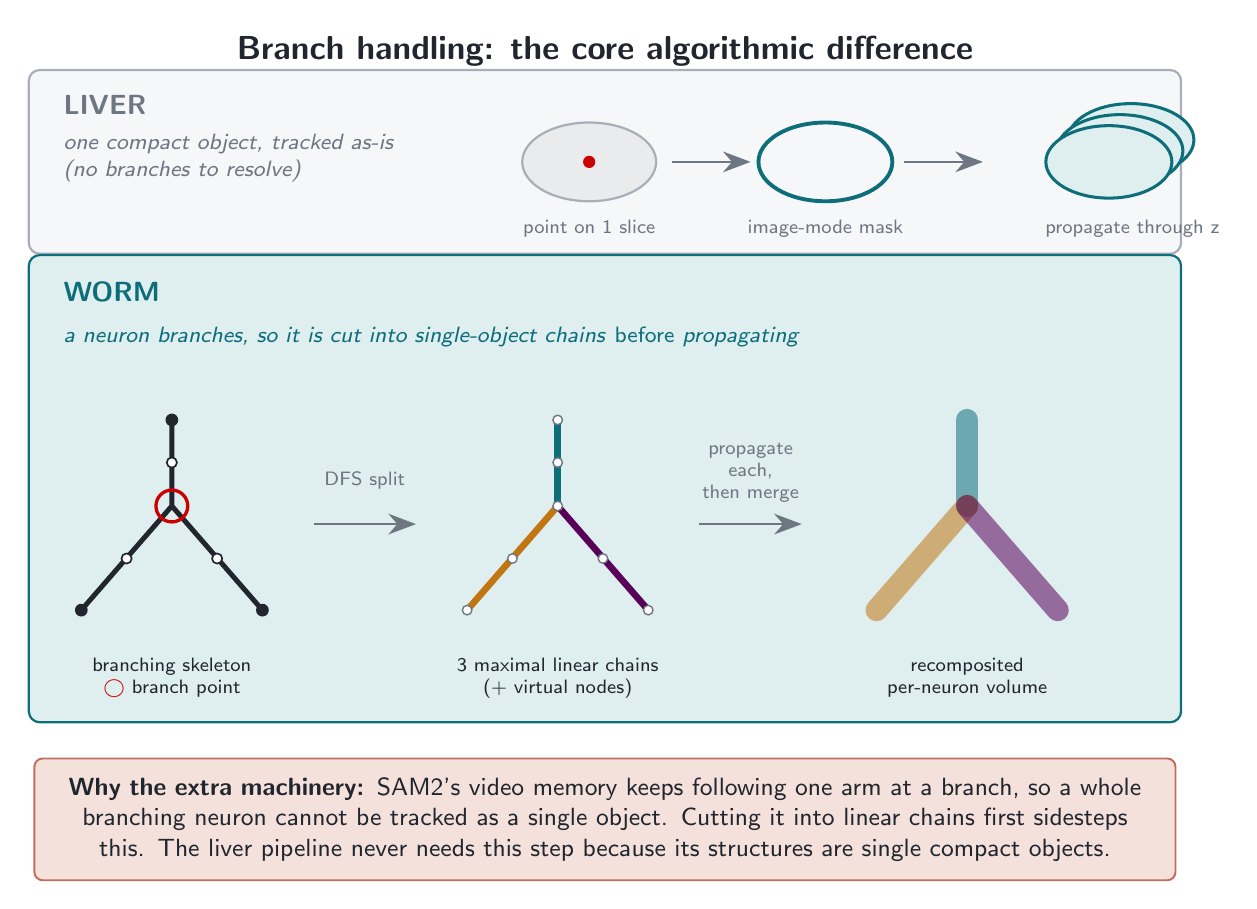
\begin{tikzpicture}[
  lbl/.style={font=\bfseries, text=inkc},
  band/.style={rounded corners=4pt, line width=0.8pt},
  arr/.style={-{Stealth[length=3.5mm]}, line width=1.0pt, spinedraw},
  capt/.style={font=\scriptsize, text=spinedraw, align=center},
  chA/.style={teald}, chB/.style={amber}, chC/.style={violet!70!black},
]

\node[align=center, font=\large\bfseries, text=inkc] at (0,4.4)
  {Branch handling: the core algorithmic difference};

% ================= LIVER band =================
\node[band, draw=liverdraw, fill=liverfill, fit={(-7.2,1.95)(7.2,4.05)}] {};
\node[lbl, text=spinedraw, anchor=west] at (-7.0,3.72) {LIVER};
\node[font=\footnotesize\itshape, text=spinedraw, anchor=west, text width=4.4cm] at (-7.0,3.05)
  {one compact object, tracked as-is (no branches to resolve)};

\begin{scope}[shift={(-0.2,3.0)}]
  % blob + point
  \fill[liverdraw!25, draw=liverdraw, line width=0.8pt] (0,0) ellipse (0.85 and 0.5);
  \fill[red!80!black] (0,0) circle (2.2pt);
  \draw[arr] (1.05,0) -- (2.05,0);
  % outlined
  \draw[teald, line width=1.4pt] (3.0,0) ellipse (0.85 and 0.5);
  \draw[arr] (4.0,0) -- (5.0,0);
  \node[capt] at (3.0,-0.85) {image-mode mask};
  % propagated stack
  \begin{scope}[shift={(6.6,0)}]
    \foreach \d in {0.28,0.14,0}{\draw[teald, line width=1.1pt, fill=tealfill] (\d,\d) ellipse (0.8 and 0.46);}
  \end{scope}
  \node[capt] at (6.9,-0.85) {propagate through z};
  \node[capt] at (0,-0.85) {point on 1 slice};
\end{scope}

% ================= WORM band =================
\node[band, draw=teald, fill=tealfill, fit={(-7.2,-4.0)(7.2,1.7)}] {};
\node[lbl, text=teald, anchor=west] at (-7.0,1.35) {WORM};
\node[font=\footnotesize\itshape, text=teald, anchor=west] at (-7.0,0.78)
  {a neuron branches, so it is cut into single-object chains \emph{before} propagating};

% ---- stage 1: branching skeleton ----
\begin{scope}[shift={(-5.5,-1.6)}, scale=1.15]
  \coordinate (R) at (0,1.15);
  \coordinate (B) at (0,0.2);
  \coordinate (La) at (-1.0,-0.95);
  \coordinate (Rb) at (1.0,-0.95);
  \draw[inkc, line width=1.8pt] (R)--(B) (B)--(La) (B)--(Rb);
  \foreach \p in {(R),(La),(Rb)}{\fill[inkc] \p circle (2pt);}
  % virtual nodes
  \foreach \p in {(0,0.68),(-0.5,-0.38),(0.5,-0.38)}{\fill[white,draw=inkc,line width=0.6pt] \p circle (1.6pt);}
  \draw[red!80!black, line width=1.2pt] (B) circle (5pt);
  \node[capt, text=inkc] at (0,-1.7) {branching skeleton\\{\color{red!80!black}$\bigcirc$} branch point};
\end{scope}

% ---- stage 2: coloured chains ----
\begin{scope}[shift={(-0.6,-1.6)}, scale=1.15]
  \coordinate (R) at (0,1.15);
  \coordinate (B) at (0,0.2);
  \coordinate (La) at (-1.0,-0.95);
  \coordinate (Rb) at (1.0,-0.95);
  \draw[chA, line width=2.4pt] (R)--(B);
  \draw[chB, line width=2.4pt] (B)--(La);
  \draw[chC, line width=2.4pt] (B)--(Rb);
  \foreach \p in {(R),(0,0.68),(B),(-0.5,-0.38),(La),(0.5,-0.38),(Rb)}{\fill[white,draw=spinedraw,line width=0.5pt] \p circle (1.5pt);}
  \node[capt, text=inkc] at (0,-1.7) {3 maximal linear chains\\(+ virtual nodes)};
\end{scope}

% ---- stage 3: per-neuron volume ----
\begin{scope}[shift={(4.6,-1.6)}, scale=1.15]
  \coordinate (R) at (0,1.15);
  \coordinate (B) at (0,0.2);
  \coordinate (La) at (-1.0,-0.95);
  \coordinate (Rb) at (1.0,-0.95);
  \begin{scope}[line cap=round, opacity=0.55]
    \draw[chA, line width=8pt] (R)--(B);
    \draw[chB, line width=8pt] (B)--(La);
    \draw[chC, line width=8pt] (B)--(Rb);
  \end{scope}
  \node[capt, text=inkc] at (0,-1.7) {recomposited\\per-neuron volume};
\end{scope}

% arrows + labels between worm stages
\draw[arr] (-3.7,-1.6) -- (-2.4,-1.6);
\node[capt] at (-3.05,-1.05) {DFS split};
\draw[arr] (1.2,-1.6) -- (2.5,-1.6);
\node[capt, text width=1.7cm] at (1.85,-0.95) {propagate each,\\then merge};

% ================= callout =================
\node[rounded corners=3pt, fill=salmonfill, draw=salmon, line width=0.7pt, align=center,
      font=\small, text=inkc, text width=14.0cm, inner sep=7pt] at (0,-5.35)
  {\textbf{Why the extra machinery:} SAM2's video memory keeps following one arm at a branch, so a
   whole branching neuron cannot be tracked as a single object. Cutting it into linear chains first
   sidesteps this. The liver pipeline never needs this step because its structures are single compact
   objects.};
\end{tikzpicture}
\end{document}
